
\section{Vorbereitung}
In dieser Übung soll das Zusammenspiel grundlegender Internetdienste veranschaulicht werden.
Hierfür werden zwei virtuelle Maschinen benötigt, die im Folgenden erstellt werden. Dabei sind folgende
Werte entsprechend zu setzen.

\scriptsize\begin{tabular}[t]{l l l l l}
\hline
Name (VMware) & Pfad (VMware) & Hostname & Benutzername & Passwort \\
\hline
srv1-0 & D:$\backslash$Austausch$\backslash$Internetdienste$\backslash$srv1-0 &
srv1-0 & admin1 & password1 \\
srv2-0 & D:$\backslash$Austausch$\backslash$Internetdienste$\backslash$srv2-0 &
srv2-0 & admin2 & password2 \\
\hline
\end{tabular}

\normalsize \subsection{Erzeugung der virtuellen Maschinen}
Im Folgenden wird die Erzeugung einer virtuellen Maschine mit VMware-Workstation exemplarisch für \textbf{srv1} gezeigt. Verfahren Sie für die Maschine \textbf{srv2} analog.
Öffnen Sie das Programm  \textbf{VMware Workstation} und wählen Sie \textbf{File$\rightarrow$New$\rightarrow$Virtual Machine} im Menü.

\begin{figure}[H]
\begin{center}
\includegraphics[width=0.85\textwidth]{screenshots/vm1.png}
\end{center}
\end{figure}

\pagebreak
Im nun erscheinenden Dialog aktivieren Sie die Option \textbf{Typical}. Danach klicken Sie auf \textbf{Next} um zur nächsten Seite des Assistenten
zu gelangen.

\begin{figure}[H]
\begin{center}
\includegraphics[width=0.85\textwidth]{screenshots/vm2.png}
\end{center}
\end{figure}

Hier muss die Option \textbf{I will install the operation system later} gewählt werden. Wieder geht es mit einem
Klick auf \textbf{Next} zur nächsten Seite.

\begin{figure}[H]
\begin{center}
\includegraphics[width=0.85\textwidth]{screenshots/vm4.png}
\end{center}
\end{figure}

\pagebreak
Wählen Sie nun als Betriebssystem \textbf{Linux} und als Version \textbf{Ubuntu} und bestätigen Sie diese
Eingaben mit einem Klick auf \textbf{Next}.

\begin{figure}[H]
\begin{center}
\includegraphics[width=0.85\textwidth]{screenshots/vm5.png}
\end{center}
\end{figure}

Geben Sie nun den Namen \textbf{srv1} und als Speicherort den Pfad \\ \textbf{D:$\backslash$Austausch$\backslash$Internetdienste$\backslash$srv1} an.

\begin{figure}[H]
\begin{center}
\includegraphics[width=0.85\textwidth]{screenshots/vm6.png}
\end{center}
\end{figure}

\pagebreak
Für die Größe der virtuellen Festplatte wählen Sie bitte \textbf{8} Gigabyte.

\begin{figure}[H]
\begin{center}
\includegraphics[width=0.85\textwidth]{screenshots/vm7.png}
\end{center}
\end{figure}

Der folgende Dialog wird jetzt mit \textbf{Finish} geschlossen.

\begin{figure}[H]
\begin{center}
\includegraphics[width=0.85\textwidth]{screenshots/vm8.png}
\end{center}
\end{figure}

\pagebreak
Als nächsten müssen noch einige Einstellungen der virtuellen Maschine bearbeitet werden. Hierzu wählen Sie
\textbf{Edit virtual machine settings}.

\begin{figure}[H]
\begin{center}
\includegraphics[width=0.85\textwidth]{screenshots/vm9.png}
\end{center}
\end{figure}
Wählen Sie nun den Eintrag \textbf{CD/DVD} und aktivieren Sie die Option \textbf{Use ISO image file}. Klicken Sie auf \textbf{Browse}
und wählen Sie die Datei \\ \textbf{D:$\backslash$Austausch$\backslash$Internetdienste$\backslash$ubuntu-10.10-server-i386.iso}.

\begin{figure}[H]
\begin{center}
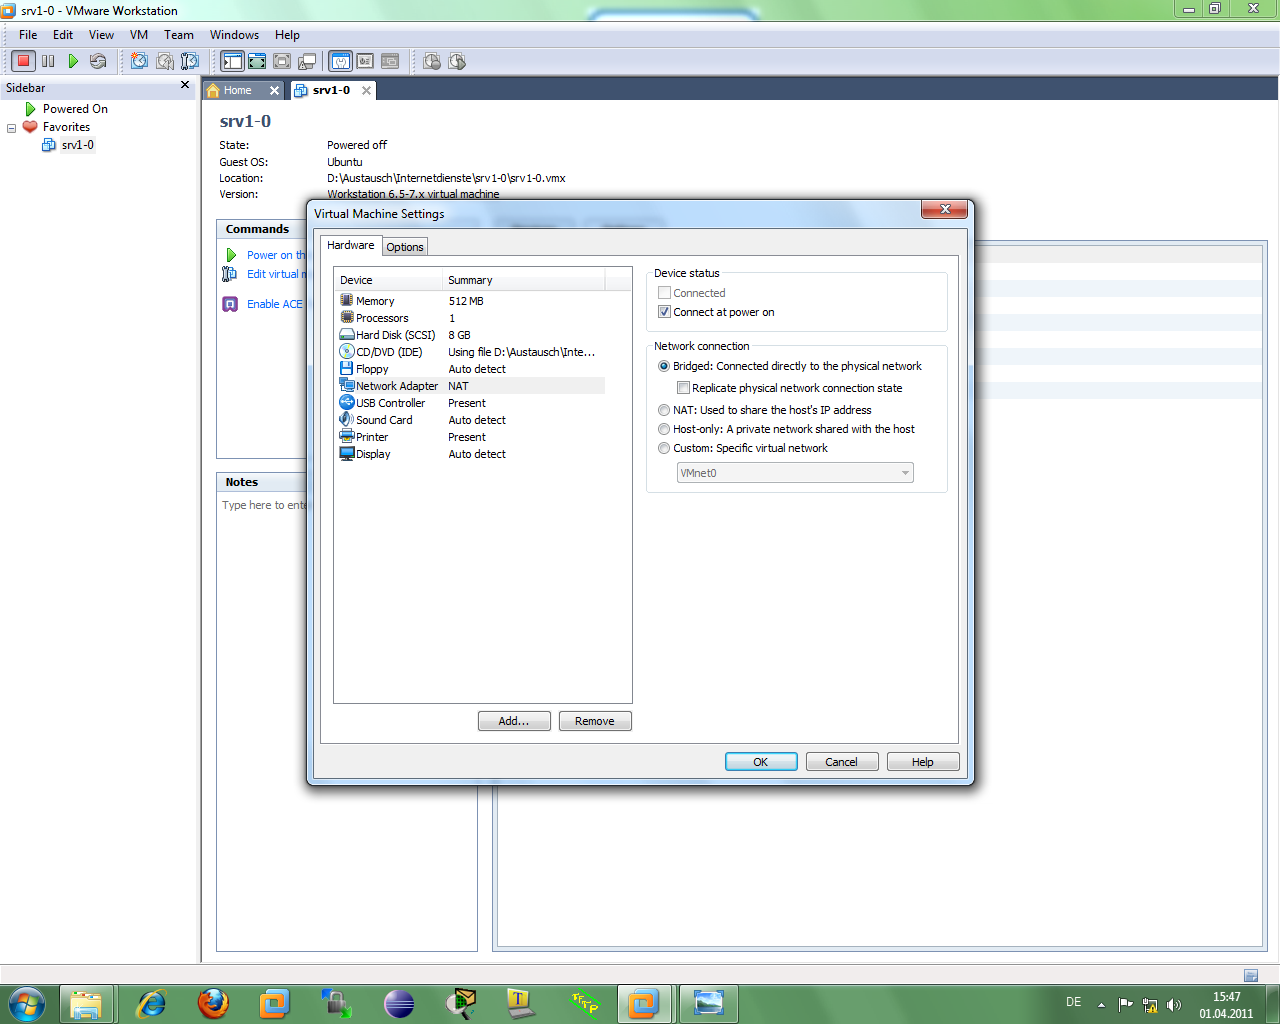
\includegraphics[width=0.85\textwidth]{screenshots/vm10.png}
\end{center}
\end{figure}

\pagebreak
Danach wählen Sie den Eintrag \textbf{Network adapter} und aktivieren die Option \textbf{Bridged}.

\begin{figure}[H]
\begin{center}
\includegraphics[width=0.85\textwidth]{screenshots/vm11.png}
\end{center}
\end{figure}

Verfahren Sie analog für den Server \textbf{srv2}.